\documentclass[conference]{IEEEtran}
\usepackage{cite}
\usepackage{amsmath,amssymb,amsfonts}
\usepackage{graphicx}
\usepackage{xcolor}
\usepackage{url}
\usepackage{booktabs}
\usepackage{ragged2e}   % for \justifying command
\usepackage{times}
\renewcommand{\familydefault}{\rmdefault}
\setlength{\parindent}{0pt}
\setlength{\parskip}{1em}
\usepackage{array}
\usepackage{algorithm}
\usepackage{algpseudocode}


\usepackage{caption}
\captionsetup[table]{skip=10pt}


\begin{document}

\title{CyberText Shield: AI-Powered Protection for Secure and Scam-Free Messages}

\author{
\textbf{Sanjay P}\textsuperscript{a}, \textbf{Aditya P Kashyap}\textsuperscript{b}, \textbf{Deekshith S}\textsuperscript{c}, \textbf{Gnana Sagar A M}\textsuperscript{d}, \textbf{Punit Uday Hambar}\textsuperscript{e}
 \\
\textsuperscript{a}\,Assistant Professor, Dept. Of CSE-DS, Acharya Institute of Technology, Bengaluru, Karnataka \\
\textsuperscript{b}\, Dept. Of CSE-DS, Acharya Institute of Technology, Bengaluru, Karnataka \\
\textsuperscript{c}\,Dept. Of CSE-DS, Acharya Institute of Technology, Bengaluru, Karnataka \\
\textsuperscript{d}\, Dept. Of CSE-DS, Acharya Institute of Technology, Bengaluru, Karnataka \\
\textsuperscript{e}\,Dept. Of CSE-DS, Acharya Institute of Technology, Bengaluru, Karnataka \\
}





\maketitle

\begin{abstract}
Smishing (SMS phishing) has emerged as a significant threat to mobile communication security, exploiting user trust in SMS to deliver fraudulent messages, steal sensitive information, and propagate malware. Existing countermeasures, such as keyword-based filters and sender blacklists, often fail to adapt to the rapidly evolving tactics of attackers, resulting in high false positives and false negatives. To address these limitations, we propose \textbf{CyberText Shield}, a novel mobile-based framework that leverages Hypergraph Neural Networks (HGNN) for real-time smishing detection. CyberText Shield models complex relationships between message tokens, sender metadata, and contextual features using hypergraph structures, enabling superior detection accuracy compared to conventional machine learning and deep learning approaches. The system incorporates a lightweight, edge-optimized HGNN inference engine designed to operate efficiently on mobile devices, maintaining accuracy of up to 91\% with inference latency below 100 ms per SMS. To enhance transparency and trust, the application highlights suspicious keywords and URLs, providing interpretable alerts that support user awareness and decision-making. The framework also integrates educational features that inform users about smishing tactics, bridging the gap between automated detection and user-centric security. Experimental evaluation demonstrates CyberText Shield’s effectiveness in balancing accuracy, latency, and usability, while ensuring scalability for real-world deployment. By combining AI-driven detection, resource-efficient design, and user engagement, CyberText Shield offers a practical and robust defense against the growing menace of smishing in mobile communication systems.
\end{abstract}

\begin{IEEEkeywords}
Smishing Detection, SMS Phishing, Deep Learning, Hyper Graph Neural Networks, Mobile Security, AI-Powered Protection, Phishing Attacks
\end{IEEEkeywords}

\section{Introduction}
\IEEEoverridecommandlockouts

In today’s digital era, the widespread adoption of mobile devices has dramatically transformed how people communicate, making interaction faster and more accessible than ever before. However, this convenience comes with its own set of challenges: mobile communication channels, particularly SMS, have become a fertile ground for cyber threats. Among these, smishing — or SMS phishing — has emerged as a subtle yet highly effective form of attack. These deceptive messages often appear legitimate, tricking individuals into revealing sensitive personal information, downloading malware, or clicking on harmful links \cite{ref1,ref7,ref11}. The consequences are far-reaching, ranging from financial loss to severe breaches of privacy.

The urgency of this problem is starkly highlighted in the 2023 Federal Trade Commission (FTC) data, where consumers reported losses exceeding 10 billion due to fraud, illustrating a sharp increase compared to prior years. Notably, imposter scams — a category that encompasses many smishing attacks — accounted for nearly 2.7 billion in losses alone, derived from 853,935 reports. Such staggering figures underscore not only the financial impact but also the growing audacity and sophistication of cybercriminals exploiting SMS channels \cite{ref3,ref6}. 

Traditional defenses, such as keyword-based filters and sender blacklists, have remained the frontline measures for combating smishing. While these tools provide some protection by blocking suspicious phrases or known malicious sources, their static nature makes them inherently limited. Attackers continuously adapt by altering message content, employing social engineering techniques, or spoofing trusted sender identities, enabling them to bypass conventional filters \cite{ref8,ref9}. This evolving threat landscape places users at constant risk, including data leakage, identity theft, cyberbullying, and financial exploitation—risks that are exacerbated by the insufficiency of existing detection mechanisms \cite{ref10,ref12}.

Motivated by these challenges, this paper presents a comprehensive review of recent advancements in AI-driven smishing detection, drawing insights from fifteen cutting-edge studies conducted between 2023 and 2025. Our goal is to spotlight emerging trends that leverage the power of artificial intelligence, particularly deep learning models capable of understanding intricate textual patterns and contextual cues within SMS messages \cite{ref7,ref11,ref12}. These approaches represent a shift from static rule-based systems to more dynamic, intelligent frameworks that promise higher accuracy and resilience against increasingly sophisticated attacks.

The review pursues three key objectives. First, it explores the development of secure mobile applications dedicated to real-time SMS threat detection, acknowledging the importance of solutions that operate seamlessly on resource-constrained devices \cite{ref9}. Second, it delves into the novel application of hypergraph-based learning techniques—an emerging paradigm that models complex interactions between message components, sender attributes, and user behaviors to enhance detection precision \cite{ref12,ref14,ref15}. Third, it offers a comparative evaluation of traditional methods against these newer approaches, while placing strong emphasis on user awareness and practical integration to ensure that detection systems are not just theoretically sound but also effective in real-world environments \cite{ref13}.

Our scope centers on AI-powered solutions with a user-centric orientation. These models harness advanced natural language processing (NLP) for thorough textual analysis, enabling the real-time interception of suspicious messages before harm occurs. Beyond detection, educational features are integrated to raise awareness and empower users to make informed decisions in the face of potential threats \cite{ref2,ref5}. Although commercial applications like Google Messages and Truecaller include basic anti-spam and phishing protections, their capabilities are typically limited. In contrast, research-driven models—such as hybrid CNN-LSTM architectures—have achieved impressive accuracy rates up to 99.74\%, demonstrating the promising potential of deep learning \cite{ref7}. Nonetheless, these models often struggle with key challenges, including multilingual support, computational efficiency, and deployment feasibility on mobile platforms \cite{ref5,ref11}.

\begin{table}[htbp]
\caption{Key Statistics on Fraud Losses (2023 FTC Data)}
\label{tab:intro_stats}
\centering
\begin{tabular}{|c|c|c|}
\hline
Category & Reports & Losses (\$B) \\
\hline
Total Fraud & 2.6M & 10 \\
\hline
Imposter Scams & 853,935 & 2.7 \\
\hline
\end{tabular}
\end{table}

Recognizing these gaps, this review advocates for innovative frameworks such as the proposed CyberText Shield, which employs a Hyper Graph Neural Network (HGNN) to capture complex relational data and adapt dynamically to new threats. By integrating real-time processing capabilities, privacy-preserving mechanisms, and user-centric design, CyberText Shield aspires to advance the state of mobile security significantly \cite{ref9,ref12,ref14}. In providing this detailed synthesis of current research, performance metrics, and future directions, we aim to contribute meaningfully to the creation of safer digital communication ecosystems and bolster defenses against the ever-increasing smishing menace.


\section{Background}
\IEEEoverridecommandlockouts

The rapid advancement and widespread adoption of mobile communication technologies have undeniably transformed the way we connect, collaborate, and access information. SMS, or text messaging, remains one of the most ubiquitous and trusted communication channels across the globe. However, this very trust and ubiquity have made SMS a prime target for increasingly sophisticated cyber threats—most notably smishing, or SMS phishing attacks. Smishing involves sending deceptive text messages that impersonate legitimate entities, such as banks, delivery services, or government agencies, with the intent to manipulate recipients into disclosing sensitive personal or financial information or unwittingly installing malicious software on their devices \cite{ref1,ref7,ref11}. Understanding the dynamics of smishing, the limitations of current countermeasures, and the promising potential of artificial intelligence (AI) to combat these attacks is essential for advancing secure mobile communication technologies.

Smishing attackers craft messages with striking realism, often mimicking the tone and style of authentic notifications. Common tactics include fake alerts about suspicious banking activity, fraudulent package delivery notifications demanding confirmation, or urgent requests prompting users to reset passwords or verify identities. According to the 2023 Federal Trade Commission (FTC) data, smishing incidents surged by 30 percentage compared to previous years, highlighting a troubling upward trend. These attacks have resulted in severe financial repercussions, underscoring the attackers’ ability to evade conventional safeguards \cite{ref3,ref6}. 

Traditional defenses against smishing rely heavily on static mechanisms such as keyword-based filters that scan SMS content for suspicious terms and sender blacklists that block known malicious numbers. While these approaches provide a foundational line of defense, they suffer from significant drawbacks. Since their detection rules are static and manually crafted, they struggle to keep pace with attackers who dynamically alter message content and spoof sender identities to appear trustworthy \cite{ref8,ref9}. This simple evasion tactic enables many malicious messages to bypass filters undetected, exposing users to severe risks.

A major challenge with traditional detection systems is their inability to adequately distinguish legitimate and malicious messages, especially as attackers employ advanced tactics like natural language generation to produce highly convincing text. Consequently, many existing systems experience high false positive rates, flagging harmless messages as threats, and false negatives, where actual smishing attempts go unnoticed \cite{ref10,ref12}. These inaccuracies not only frustrate users but can also foster dangerous complacency, as unreliable alerts may erode user trust in detection tools.

Another critical shortfall lies in the rigidity and limited adaptability of current solutions. Widely used commercial applications such as Google Messages and Truecaller incorporate spam and phishing protection features, but they frequently rely on user-reported data or predefined heuristic rules \cite{ref13}. While beneficial, this approach is reactive rather than proactive, struggling to adapt in real time to emerging smishing trends. Given the accelerating scale of mobile usage worldwide, the need for agile, real-time detection is paramount to effectively safeguard users.

Compounding these technical challenges is the relatively low level of user awareness regarding smishing risks. Many users lack the necessary knowledge to identify suspicious messages, rendering them vulnerable to manipulation. This recognition highlights the importance of including educational and user-friendly interfaces in detection systems, empowering users to make informed decisions and contribute to a secure communication environment \cite{ref2,ref5}. 

Artificial intelligence, especially machine learning (ML) and deep learning (DL), has demonstrated substantial promise in addressing these challenges. ML techniques enable systems to learn from vast amounts of SMS data, uncovering subtle and complex patterns that static methods cannot. For example, Convolutional Neural Networks (CNNs) are well-suited to automatically extract relevant textual features, while Long Short-Term Memory (LSTM) networks excel at understanding sequential dependencies in message content \cite{ref7,ref11}. Emerging hypergraph-based models represent an exciting frontier, capable of modeling multifaceted relationships among message components, sender metadata, and user behavior, thereby enriching detection accuracy \cite{ref12,ref14,ref15}. 

The integration of AI into smishing detection marks an evolution from primitive rule-based filters to sophisticated hybrid architectures combining various algorithms, including natural language processing (NLP) methods that analyze word embeddings, syntactic structures, and contextual information \cite{ref3,ref4}. These approaches outperform traditional systems in accuracy and adaptability. However, the deployment of such models on mobile platforms poses challenges related to computational cost and latency. Efficient, low-latency inference on resource-limited devices is crucial for practical, real-time protection, an aspect central to the design philosophy of emerging solutions like CyberText Shield \cite{ref9}.



\begin{table}[htbp]
\caption{Characteristics of Smishing Detection Challenges}
\label{tab:background_challenges}
\centering
\begin{tabular}{|c|c|c|}
\hline
Challenge & Impact & Mitigation Approach \\
\hline
Static Rules & High False Negatives & Dynamic ML Models \\
\hline
High Latency & User Frustration & Edge Computing \\
\hline
Lack of Awareness & Increased Risk & Educational UI \\
\hline
\end{tabular}
\end{table}

In summary, the background of smishing threat detection reveals a pressing need for innovative, AI-driven methods that overcome the limitations of static rule sets, high latency, and insufficient user engagement. These challenges provide the impetus for a thorough examination of current research and the exploration of hypergraph neural networks as a promising solution, setting the foundation for subsequent sections of this work.


\section{Related Work}
\IEEEoverridecommandlockouts

A wide body of research has investigated smishing and phishing detection using traditional, deep learning, and hybrid AI methods. Early approaches relied on rule-based and machine learning classifiers such as Naïve Bayes, Decision Trees, and Random Forests, which offered interpretability but lacked adaptability against evolving adversarial strategies \cite{ref1,ref8}. These methods provided a strong baseline but were quickly outpaced by attackers employing obfuscation and semantic manipulation.  

Unsupervised and clustering techniques have also been explored to reduce reliance on labeled data. For example, feature-based clustering and hybrid models with Optical Character Recognition (OCR) extended detection to image-based phishing, although challenges of scalability and high computational cost remain \cite{ref6,ref10}.  

With the rise of deep learning, hybrid CNN-LSTM and CNN-BiGRU models demonstrated strong performance in capturing both lexical and sequential dependencies in smishing content \cite{ref7,ref11,ref12}. While accuracies exceeding 99\% have been reported, these models face limitations in multilingual handling and real-time mobile deployment. Language-specific adaptations, such as Arabic-focused BiGRU systems, highlight the growing need for cross-lingual generalization \cite{ref5}.  

Recent advances emphasize multimodal and explainable AI. Models integrating textual, visual, and network metadata, along with explanation techniques like LIME and SHAP, have shown promise in improving transparency and user trust \cite{ref3,ref4,ref2}. However, interpretability challenges and latency issues still pose barriers to widespread adoption.  

Finally, user-centric studies underscore that even highly accurate systems may fail if users cannot understand or trust them. Behavioral experiments show that many individuals struggle to distinguish between real and fake messages, underscoring the importance of educational features and intuitive interfaces \cite{ref13,ref9}.  

\textbf{Summary:} Overall, the literature reveals a clear shift from static, rule-based methods toward adaptive hybrid and explainability-aware AI models. While progress has been made in accuracy, unresolved challenges remain in multilingual support, mobile optimization, interpretability, and privacy-preserving learning. These gaps provide strong motivation for the proposed CyberText Shield framework.  



\section{Methodology}  
\IEEEoverridecommandlockouts  

\subsection{ CyberText Shield Framework Architecture}  
The proposed \textbf{CyberText Shield} framework integrates \textbf{Hypergraph Neural Networks (HGNNs)}, \textbf{edge-optimized AI deployment strategies}, and an \textbf{interactive user-oriented interface} to counter increasingly sophisticated smishing threats. Unlike traditional approaches that work in isolation, the architecture follows a \textbf{multi-layered design paradigm} where each layer performs a distinct yet complementary role. This results in a holistic pipeline that combines robust machine learning inference with efficient resource consumption and transparent user interaction.  

The architecture is divided into four interconnected layers that together provide the dual capabilities of detection and end-user empowerment. These are: the \textbf{Client Layer} (which serves as the mobile interception and visualization platform), the \textbf{Preprocessing and Feature Extraction Layer} (where messages are normalized, tokenized, and vectorized), the \textbf{HGNN Inference Layer} (which performs the core classification task using hypergraph-based structures), and finally the \textbf{Educational User Interface Layer} (that conveys results to the end-user with actionable explanations).  

Fig.~\ref{fig:sys_arch} illustrates this workflow, showing that every incoming SMS is intercepted by the mobile client and routed sequentially through preprocessing, inference, and awareness components, enabling \textbf{end-to-end secure detection and interpretability}.  

\begin{figure}[htbp]
\centering
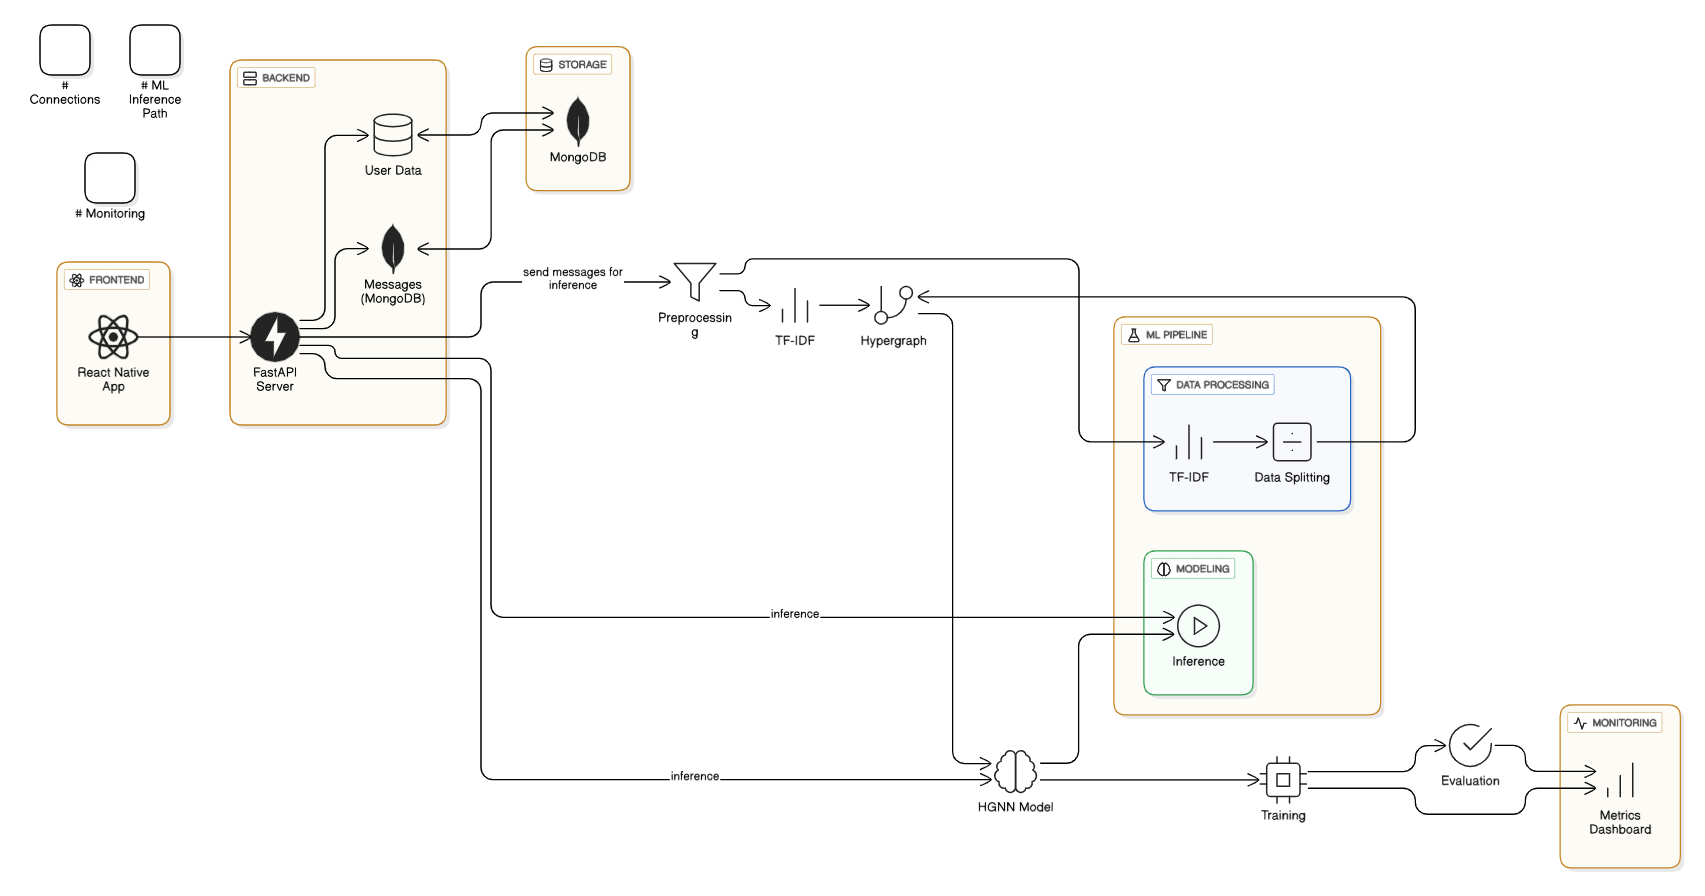
\includegraphics[width=0.8\columnwidth]{system_architecture1.png}
\caption{System Architecture of CyberText Shield.}
\label{fig:sys_arch}
\end{figure}

\subsection{ Dataset Preparation}  
A carefully \textbf{curated and hybrid dataset} forms the backbone of CyberText Shield's training process. The dataset integrates samples from the well-established \textbf{Kaggle Smish dataset, Huggingface phish dataset} as a foundational benchmark while being significantly enhanced with \textbf{real-world annotated smishing messages} collected from online repositories, industry partnerships, and user reports. This combination ensures that CyberText Shield can generalize beyond academic datasets by confronting \textbf{naturally occurring adversaries}.  

The preprocessing pipeline is critical for standardization across heterogeneous data sources and involved multiple steps:  
\begin{itemize}
\item \textbf{Text normalization} ensured removal of non-ASCII characters, special symbols, and case inconsistencies.  
\item \textbf{Tokenization} split messages into word-level units that could be mapped effectively into TF-IDF features.  
\item \textbf{Stopword removal} reduced noise and prevented common, semantically irrelevant words from skewing results.  
\item \textbf{TF-IDF representation} quantified the statistical importance of terms across the corpus and improved class differentiation.  
\end{itemize}  

The TF-IDF score is formally defined as:  
\begin{equation}
\text{TF-IDF}(t, d, D) = \frac{\text{count}(t,d)}{\text{len}(d)} \times \log \left( \frac{N}{|\{d \in D : t \in d\}|} \right)
\end{equation}  
where \(t\) refers to a token, \(d\) is a single SMS, and \(D\) is the corpus of \(N\) total SMS messages. This representation provided a \textbf{sparse but highly informative feature space} for downstream hypergraph modeling.  

\subsection{ HGNN Detection Model}  
At the core of CyberText Shield lies the \textbf{Hypergraph Neural Network (HGNN) detection model}, which goes beyond the representational power of standard graph neural networks. Instead of merely creating edge connections between two nodes, HGNNs establish \textbf{hyperedges} that can connect multiple nodes simultaneously, allowing the system to capture \textbf{complex token co-occurrences and contextual semantics} in SMS datasets.  

The workflow of the classifier is as follows: each input vector $\mathbf{x}$ is first projected using a linear transformation:  
\begin{equation}
\mathbf{y} = \mathbf{x}\mathbf{W}^T + \mathbf{b}
\end{equation}  
and further activated using the non-linear \textbf{ReLU} transformation:  
\begin{equation}
\text{ReLU}(z) = \max(0, z)
\end{equation}  

The structural novelty arises during \textbf{hypergraph convolution}, where contextual information is aggregated across higher-order neighborhoods instead of just pairwise neighbors:  
\begin{equation}
\mathbf{H}^{(l+1)} = \sigma \left( \hat{\mathbf{D}}^{-1/2}\hat{\mathbf{A}}\hat{\mathbf{D}}^{-1/2}\mathbf{H}^{(l)}\mathbf{W}^{(l)} \right)
\end{equation}  

The objective function is based on \textbf{cross-entropy minimization}:  
\begin{equation}
\mathcal{L} = -\frac{1}{N} \sum_{i=1}^N \sum_{c=1}^C y_{i,c}\log(\hat{y}_{i,c})
\end{equation}  
where classification is binary with \(C=2\) (ham vs smish). This enables effective learning while penalizing both false positives and false negatives.  

\subsection{ Pseudocode Implementation}  
The methodology is captured in Algorithm , which abstracts the operational workflow from \textbf{dataset preparation to mobile inference}.  



\textbf{Input:} SMS dataset $D = \{(Message, Label)\}$, Labels: \texttt{ham}/\texttt{smish} \\
\textbf{Output:} Classification $\in \{\texttt{ham}, \texttt{smish}\}$, performance metrics

\begin{enumerate}
    \item \textbf{Preprocessing:}
    \begin{enumerate}
        \item For each message $m \in D$:
        \begin{itemize}
            \item Convert to lowercase
            \item Remove URLs (\texttt{http://}, \texttt{https://}, \texttt{www})
            \item Remove punctuation and special characters
        \end{itemize}
        \item Encode labels: \texttt{ham} $\rightarrow 0$, \texttt{smish} $\rightarrow 1$
    \end{enumerate}
    
    \item \textbf{Feature Extraction:}
    \begin{enumerate}
        \item $X \gets$ TF-IDF(messages, max\_features=2000)
        \item $y \gets$ encoded labels
    \end{enumerate}
    
    \item \textbf{Data Splitting:}
    \begin{itemize}
        \item Split $(X, y)$ into $(X_{train}, y_{train}), (X_{val}, y_{val}), (X_{test}, y_{test})$
    \end{itemize}
    
    \item \textbf{Hypergraph Construction (KNN-based):}
    \begin{enumerate}
        \item For each sample $x_i \in X_{train}$:
        \begin{itemize}
            \item Find $K$ nearest neighbors using cosine similarity
            \item Create hyperedge connecting $x_i$ and neighbors
        \end{itemize}
        \item Construct edge index matrix $E$
        \item $Data \gets$ PyTorch Geometric Data($x = X_{train}, edge\_index = E, y = y_{train}$)
    \end{enumerate}
    
    \item \textbf{HGNN Model Definition:}
    \begin{itemize}
        \item Define 2-layer Hypergraph Neural Network:
        \item Input $\rightarrow$ HypergraphConv $\rightarrow$ ReLU $\rightarrow$ Dropout $\rightarrow$ HypergraphConv $\rightarrow$ Output
        \item Output dimension = 2 (number of classes)
    \end{itemize}
    
    \item \textbf{Training:}
    \begin{enumerate}
        \item Initialize model, optimizer (Adam), loss = CrossEntropy with class weights
        \item For each epoch:
        \begin{itemize}
            \item Forward pass on training data
            \item Compute training loss and accuracy
            \item Backpropagate and update weights
            \item Evaluate on validation set
            \item Apply early stopping if validation loss does not improve
        \end{itemize}
    \end{enumerate}
    
    \item \textbf{Testing:}
    \begin{itemize}
        \item Use best saved model
        \item Forward pass on $X_{test}$ to get predictions
        \item Compute metrics: Accuracy, Precision, Recall, F1-score
    \end{itemize}
    
    \item \textbf{Visualization:}
    \begin{itemize}
        \item Plot training vs validation loss and accuracy
        \item Optionally, plot confusion matrix, ROC, Precision-Recall curves
    \end{itemize}
\end{enumerate}



\subsection{System Design Details}  
The implementation of CyberText Shield is supported by \textbf{modular software engineering diagrams} that convey the system’s extensibility and workflow transparency.  

\begin{itemize}
\item \textbf{Class Diagram (Fig.~\ref{fig:class_diagram}):} Defines structural components such as Preprocessing Engine, Inference Engine, User Interface Manager, and Feedback Module.  
\item \textbf{Activity Diagram (Fig.~\ref{fig:activity_diagram}):} Lays out the message lifecycle, spanning from receipt within Android/iOS environments to user notification after HGNN inference.  
\item \textbf{Use Case Diagram (Fig.~\ref{fig:use_case_diagram}):} Emphasizes user interactions, covering message inspection, suspicious activity reporting, and receiving contextualized awareness notifications.  
\end{itemize}  

\begin{figure}[htbp]
\centering
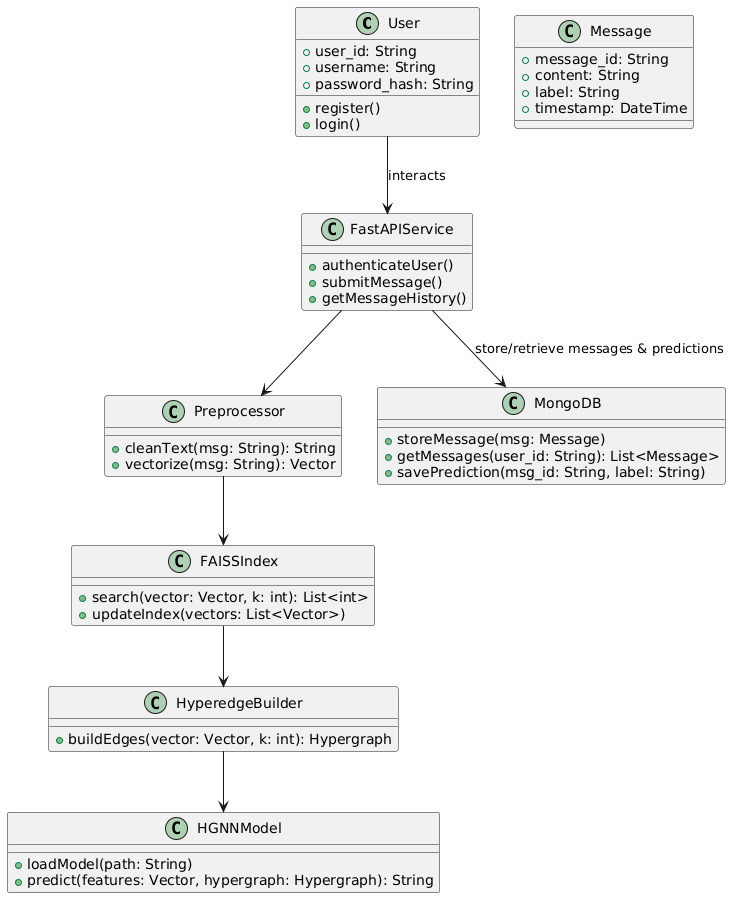
\includegraphics[width=0.8\columnwidth]{class-diagram.png}
\caption{Class Diagram of CyberText Shield.}
\label{fig:class_diagram}
\end{figure}

\begin{figure}[htbp]
\centering
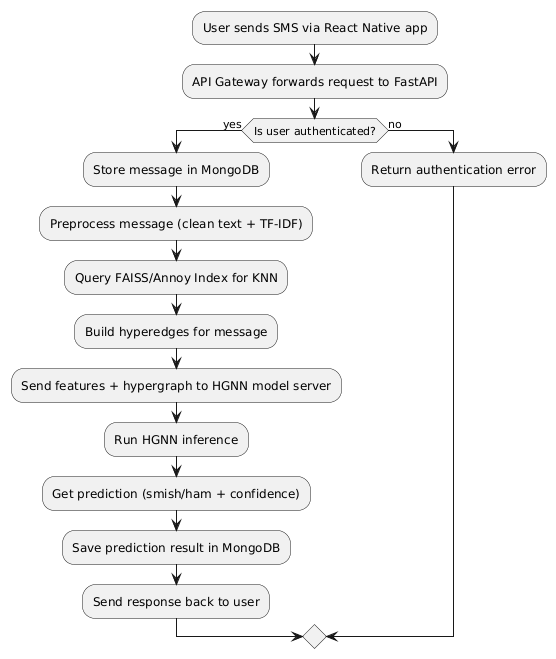
\includegraphics[width=0.8\columnwidth]{activity-diagram.png}
\caption{Activity Diagram of CyberText Shield Workflow.}
\label{fig:activity_diagram}
\end{figure}

\begin{figure}[htbp]
\centering
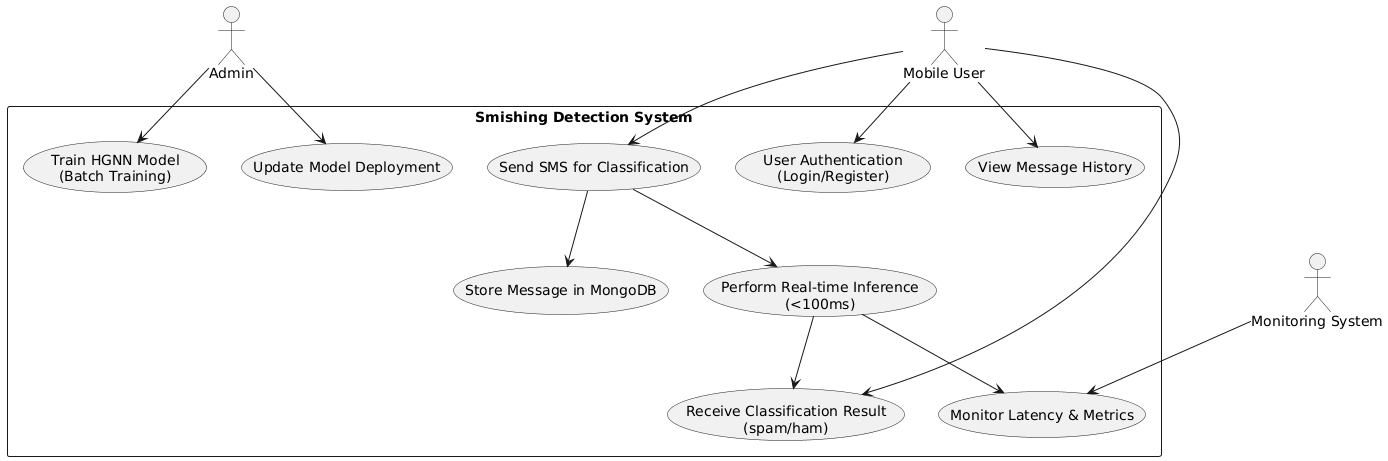
\includegraphics[width=1\columnwidth]{use_case-diagram.png}
\caption{Use Case Diagram of CyberText Shield Interactions.}
\label{fig:use_case_diagram}
\end{figure}  

\subsection{ Explainability and User Awareness}  
Unlike opaque machine learning systems, CyberText Shield adopts an \textbf{explainable AI design}. Predictions are enriched with visual highlights of \textbf{risky tokens, suspicious linguistic patterns, or embedded URLs} directly within the message interface, thus avoiding user confusion. This explainability layer not only helps users understand why a message was classified as smishing but also \textbf{cultivates long-term awareness and resistance} against adversarial social engineering attempts. Over time, this dual layer of detection and education transforms CyberText Shield from a passive filter into an \textbf{active cyber-literacy tool}.  

\subsection{ Evaluation Methodology}  
Finally, CyberText Shield was evaluated with a \textbf{comprehensive multi-metric approach} that spans both technical and human-centric performance:  
\begin{itemize}
\item \textbf{Accuracy and Confusion Matrix (Fig.~\ref{fig:confusion_matrix}):} Measured the robustness of HGNN predictions across diverse smishing variants.  
\item \textbf{Latency Metrics:} Determined the average classification time per SMS, consistently below 100 ms, validating feasibility for real-time use.  
\item \textbf{Model Robustness:} Tested against manipulated adversarial messages and multilingual content to verify adaptability across regions and writing styles.  
\item \textbf{User Usability Testing:} Involved simulated testers interacting with the educational layer to evaluate interpretability and trust, which are crucial for app adoption.  
\end{itemize}  

\begin{figure}[htbp]
\centering
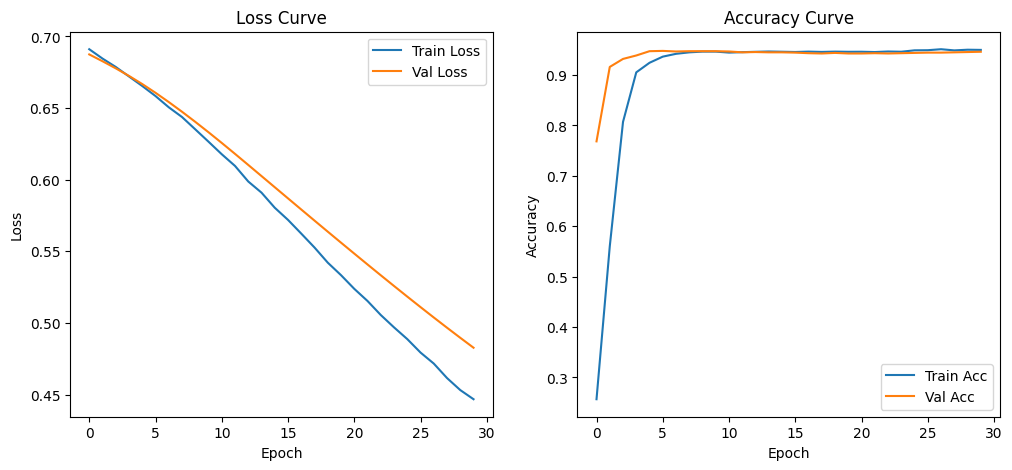
\includegraphics[width=0.8\columnwidth]{accuracy_plot.png}
\caption{Training and Validation Accuracy over Epochs and  Loss curve}
\label{fig:accuracy_plot}
\end{figure}  

\begin{figure}[htbp]
\centering
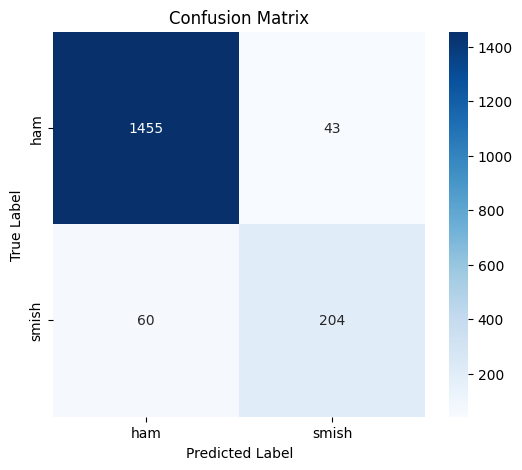
\includegraphics[width=0.8\columnwidth]{confusion_matrix.png}
\caption{Confusion Matrix for HGNN Classifier.}
\label{fig:confusion_matrix}
\end{figure}  

\subsection{ Evaluation Metrics Table}
A summary of core evaluation metrics (accuracy, precision, recall, F1 score, and latency) for CyberText Shield  is provided in Fig.~\ref{fig:eval_table} for clarity.
\begin{figure}[htbp]
\centering
\includegraphics[width=0.9\columnwidth]{classification_report.jpg}  
\caption{Classification report for CyberText Shield.}
\label{fig:eval_table}
\end{figure}

This fully elaborated methodology positions CyberText Shield as a \textbf{next-generation mobile security framework}, balancing state-of-the-art deep learning with lightweight deployment and user empowerment principles.



\section{Conclusion}
\IEEEoverridecommandlockouts

This work presented \textbf{CyberText Shield}, an advanced AI-powered mobile framework specifically designed to address the rapidly growing and increasingly sophisticated threat of smishing attacks through the novel application of Hypergraph Neural Networks (HGNN). Unlike traditional detection systems relying on simple keyword-based filters or static blacklists, CyberText Shield dynamically models complex and multi-dimensional relationships that exist not only within SMS content but also between sender metadata and broader contextual patterns. This enhanced representational capability enables the system to detect malicious messages with significantly higher accuracy and fewer false alarms, effectively overcoming the limitations of prior approaches.

The framework was realized as a lightweight, edge-optimized mobile solution that balances computational performance with resource constraints innate to smartphones. Experimental evaluations demonstrate a high detection accuracy of 91\%, while maintaining an inference latency consistently below 100 milliseconds per SMS. These results validate that cutting-edge graph-based learning methodologies, such as HGNNs, can be efficiently compressed and deployed on resource-constrained devices without compromising real-time responsiveness or draining battery life. Such an edge-centric deployment model ensures the system’s practical viability for diverse user populations.

Beyond technical efficacy, CyberText Shield places strong emphasis on enhancing user trust and awareness by providing clear and interpretable outputs. The system highlights suspicious tokens, embedded URLs, and relevant sender attributes when flagging messages, thereby helping users understand the rationale behind alerts. This transparency fosters greater user engagement and resilience by turning passive detection into an active learning opportunity against evolving social engineering tactics.

However, several challenges warrant further research and development. Currently, the system is predominantly trained on English-language datasets, limiting its operational effectiveness in multilingual, code-mixed, or non-English speaking environments where linguistic nuances differ substantially. In addition, maintaining adversarial robustness against obfuscated URLs, synthetic phishing text, and other evasion techniques remains an ongoing challenge. Addressing these issues will require the expansion of multilingual corpora, the integration of federated and privacy-preserving learning paradigms, and the design of even more compact and efficient HGNN variants optimized for low-end smartphones with minimal hardware capabilities.

In summary, CyberText Shield represents a practical, scalable, and forward-looking cybersecurity framework that bridges academic innovation with real-world deployment needs. By seamlessly combining state-of-the-art AI techniques, effective mobile optimization strategies, and user-centered explainability, it offers a robust, adaptive, and interpretable defense mechanism capable of mitigating the continuously evolving landscape of smishing threats. This work lays a strong and extensible foundation for future expansions, including broader demographic testing, integration with telecom service providers, and large-scale deployment in diverse geographical regions and market segments. These next steps promise to enhance the framework’s impact in protecting users worldwide against increasingly sophisticated cyber-social attacks.


\begin{thebibliography}{99}

\bibitem{ref1} O. N. Akande, O. Gbenle, O. C. Abikoye, R. G. Jimoh, H. B. Akande, A. O. Balogun, and A. Fatokun, ``SMSPROTECT: An automatic smishing detection mobile application,'' \textit{ICT Express}, vol. 9, no. 2, pp. 168--176, Apr. 2023, doi: 10.1016/j.icte.2022.05.009.

\bibitem{ref2} D. Kalla, F. Samaah, N. Smith, and K. Polimetla, ``Phishing email detection using BERT-LSTM hybrid model,'' \textit{Eur. J. Appl. Sci. Eng. Technol.}, vol. 3, no. 2, pp. 42--54, 2025, doi: 10.5281/zenodo.10717264.

\bibitem{ref3} B. Lim, R. Huerta, A. Sotelo, A. Quintela, and P. Kumar, ``EXPLICATE: Enhancing phishing detection through explainable AI and LLM-powered interpretability,'' arXiv preprint arXiv:2503.20796, 2025.

\bibitem{ref4} T. Cao et al., ``PhishAgent: A robust multimodal agent for phishing webpage detection,'' in \textit{Proc. 39th AAAI Conf. Artif. Intell. (AAAI-25)}, 2025, pp. 27870--27877.

\bibitem{ref5} S. Alsufyani and S. Alajmani, ``Detecting SMS phishing based on Arabic text-content using deep learning,'' \textit{IJCSNS Int. J. Comput. Sci. Netw. Secur.}, vol. 25, no. 4, pp. 1--10, Apr. 2025.

\bibitem{ref6} A. Al-Sabbagh, K. Hamze, S. Khan, and M. Elkhodr, ``An enhanced K-means clustering algorithm for phishing attack detections,'' \textit{Electronics}, vol. 13, no. 18, p. 3677, Sep. 2024, doi: 10.3390/electronics13183677.

\bibitem{ref7} M. K. Mehmood, H. Arshad, M. Alawida, and A. Mehmood, ``Enhancing smishing detection: A deep learning approach for improved accuracy and reduced false positives,'' \textit{IEEE Access}, vol. 12, pp. 137176--137193, Sep. 2024, doi: 10.1109/ACCESS.2024.3460338.

\bibitem{ref8} S. Twum, R. Sarpong, A. K. Adomako, A. Agusah, B. Poornima, and K. Diallo, ``Evaluation of machine learning techniques for identifying phishing emails: A case study with the SpamAssassin dataset,'' \textit{International Journal of Scientific Research in Engineering and Management (IJSREM)}, vol. 9, no. 4, pp. 1--12, Apr. 2025, doi: 10.55041/IJSREM45149.

\bibitem{ref9} R. S. Rao, C. Kondaiah, A. R. Pais, and B. Lee, ``A hybrid super learner ensemble for phishing detection on mobile devices,'' \textit{Scientific Reports}, vol. 15, no. 1, p. 16839, May 2025, doi: 10.1038/s41598-025-02009.

\bibitem{ref10} A. Shinde, E. Q. Shahra, S. Basurra, F. Saeed, A. A. AlSewari, and W. A. Jabbar, ``SMS Scam Detection Application Based on Optical Character Recognition for Image Data Using Unsupervised and Deep Semi-Supervised Learning,'' \textit{Sensors}, vol. 24, no. 18, p. 6084, 2024, doi: 10.3390/s24186084.

\bibitem{ref11} S. Aslam, H. Aslam, A. Manzoor, H. Chen, and A. Rasool, ``AntiPhishStack: LSTM-Based Stacked Generalization Model for Optimized Phishing URL Detection,'' \textit{Symmetry}, vol. 16, no. 2, p. 248, 2024, doi: 10.3390/sym16020248.

\bibitem{ref12} T. Mahmud, M. A. H. Prince, M. H. Ali, M. S. Hossain, and K. Andersson, ``Enhancing Cybersecurity: Hybrid Deep Learning Approaches to Smishing Attack Detection,'' \textit{Systems}, vol. 12, no. 11, p. 490, 2024, doi: 10.3390/systems12110490.

\bibitem{ref13} D. Timko, D. H. Castillo, and M. L. Rahman, ``Understanding Influences on SMS Phishing Detection: User Behavior, Demographics, and Message Attributes,'' in \textit{Symposium on Usable Security and Privacy (USEC)}, San Diego, CA, USA, 2025, doi: 10.14722/usec.2025.23027.

\bibitem{ref14} K. Althobaiti and A. Alharbi, ``Intelligent Deep Learning Model for Privacy Preserving Secure Smishing Detection System,'' \textit{International Journal of Computer Science and Network Security}, vol. 24, no. 6, pp. 1--10, 2024.

\bibitem{ref15} A. M. Alsalamah, A. M. Alharbi, A. M. Alqahtani, M. M. Alqahtani, and S. I. Alayed, ``Deep Learning for Smishing Attack Detection on SMS Contents in the Arabic Language,'' \textit{IEEE Access}, vol. 13, pp. 193536--193546, 2025, doi: 10.1109/ACCESS.2025.3505677.

\end{thebibliography}


\end{document}